% 144-01(144쪽) — 색칠한 삼각형 ABC(B 왼쪽 아래 · C 오른쪽 아래 · A 위) · AB=4, ∠B=30°, BC=6.
% 스캔 그림이라 화질이 낮아 TikZ 로 다시 그렸다. 라벨은 원문에 있는 A·B·C·4·30°·6 만 두고 넓이(답)는 적지 않는다.
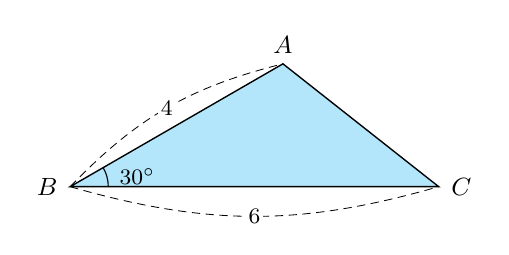
\begin{tikzpicture}[scale=0.78, line width=0.5pt]
  \coordinate (B) at (0,0);
  \coordinate (C) at (6,0);
  \coordinate (A) at (3.464,2);
  \fill[cyan!30] (A) -- (B) -- (C) -- cycle;
  \draw (A) -- (B) -- (C) -- cycle;
  \draw[line width=0.4pt] ([shift=(0:0.62)]B) arc (0:30:0.62);
  \node[right=1pt, font=\footnotesize] at ([shift=(15:0.62)]B) {$30^\circ$};
  \node[above=0pt, font=\small] at (A) {$\pt{A}$};
  \node[left=1pt, font=\small] at (B) {$\pt{B}$};
  \node[right=1pt, font=\small] at (C) {$\pt{C}$};
  \draw[densely dashed, line width=0.3pt] (B)
    to[bend left=16] node[midway, fill=white, inner sep=1pt, font=\footnotesize] {$4$} (A);
  \draw[densely dashed, line width=0.3pt] (B)
    to[bend right=16] node[midway, fill=white, inner sep=1pt, font=\footnotesize] {$6$} (C);
\end{tikzpicture}
